\chapter{Background}\label{chap:background}


This chapter is devoted for introducing and familiarizing the reader to the theoretical concepts behind this project, and give the reader a background on the theorem prover E as well. So it will include the following sections:
	\begin{itemize}
		\item A background on \ac{fol} in section %TODO add a reference
		\item A background on \ac{epr} in section %TODO add a reference
		\item A background on \ac{atp} in section %TODO add a reference
		\item A background on E in section %TODO add a reference
		\item A background on Problem set in section %TODO add a reference
	\end{itemize}


\section{Background on first order logic topics} \label{sec:c2s1}

\ac{fol}, which is also known as first order predicate logic, is an expressive logic that allows us to formulate most of our spoken language sentences in a defined way such that it could be further handled with rules such as simplification, inference rules, etc.\\*
We could represent formulas in \ac{fol} in so many forms. So \ref{sub:c2s1s1} will be devoted to that part of background.\newline
Moreover, in general the universe of \ac{fol} is infinite because of the existence of the quantifiers and function terms. So in \ref{sub:c2s1s2} some topics related to that property will be mentioned including Herbrand Universe.\newline    
Also this project is concerned to a specific class of \ac{fol} its calculus named \ac{epr}, and this will be discussed in \ref{sub:c2s1s4}.

\subsection{Different forms of \ac{fol}}\label{sub:c2s1s1}
\ac{fol} can be represented in different forms. Even some algorithms need to work with specific one.
Moreover, there are some procedures that could transform a formula from one form to another.
Here in this part, we will discuss the most important forms and the relevant ones to the project.
\newline
1- general form\newline 
2- clausal normal form\newline
3- prenex normal form\newline
4- skolem normal form

\subsubsection{General Form}
General form

\subsubsection{Clausal normal form}
\ac{cnf}

\subsubsection{Prenex normal form}
\ac{pnf}

\subsubsection{Skolem normal form}
\ac{snf}

\subsection{The universe of \ac{fol}}\label{sub:c2s1s2}
Discuss the infinity of the universe in general.\newline
And then mention the Herbrand Universe. 

\subsection{Skolemization}\label{sub:c2s1s3}
Skolemization is the step that transforms \ac{pnf} formulas into \ac{snf}.
In which all the existentially quantified variables are removed and replaced by some function terms and its arguments are all the universally quantified variables appeared before the one in concern.\\
Example for a formula in \ac{pnf}:\newline
\begin{displaymath}
\exists W \forall X \forall Y \exists Z  \left(P(a,W,X,Y,Z)\right).  
\end{displaymath}\newline
After it transformed into \ac{snf}:\newline
\begin{displaymath}
\forall X \forall Y  \left(P(a,b,X,Y,f(X,Y))\right).  
\end{displaymath}

%TODO add link to the algorithm of the transformation in the appendix. 

\subsection{What is \ac{epr}}\label{sub:c2s2s1}
\acf{epr} or sometimes known as Bernays-Sch\"onfinkel class is a fragment of \acf{fol} in which all of its formulas follow the following format:

\begin{lstlisting}[caption=Format of \ac{epr} formula,label={lst:epr_format},breaklines=true,mathescape,frame=single]
                          $\exists *$ $\forall *$ $F$
  where $F$ is the formula.
  Moreover, $F$ has no proper functions symbols (all functions present are nullary ones "constants").
\end{lstlisting}

\ac{epr} fragment has a huge number of applications, e.g. Planning and Verifcation. 


\subsection{Example on \ac{epr}}\label{sub:c2s2s2}
Example for a formula in \ac{epr}:

\begin{lstlisting}[caption=Example for an \ac{epr} formula,breaklines=true,escapeinside={(*}{*)},frame=single]
(* \begin{displaymath}
		\exists X \exists Y \forall Z  \left(P(a,X,Y,Z)\right).
	\end{displaymath} *)
\end{lstlisting}


Keeping \ref{lst:epr_format} in mind, this will make every skolemized formula that originally was in \ac{epr} format have no proper function symbols. After transforming the above equation, it will be:

\begin{lstlisting}[caption=Example for a skolemized \ac{epr} formula,breaklines=true,escapeinside={(*}{*)},frame=single]
(* \begin{displaymath}
	\forall Z \left( P(a,b,c,Z) \right).
	\end{displaymath} *)
\end{lstlisting}



\subsection{Decidability and Universe of \ac{epr}}\label{sub:c2s2s3}
Since the domain of \ac{epr} formulas contains only constants, and the number of constants in a formula is finite. So Herbrand universe of \ac{epr} formulas is finite. From that we could prove that \ac{epr} fragment is a decidable fragment in \ac{fol}, because of the finite number of ground interpretations it can have.


\subsection{Equality in \ac{epr}}\label{sub:c2s2s4}
As we have mentioned before that \ac{epr} formulas will never contain proper function symbols. So terms will be one of two options:
\begin{itemize}
	\item constant
	\item variable
\end{itemize}


And since Equality may be added to \ac{fol} as discussed in subsection \ref{sub:c2s2s3}, then we should consider the case if the formulas are from the \ac{epr} fragment. Equations are in the following form $t1$ $\approx$ $t2$, where t1 and t2 are terms. And since terms in \ac{epr} are only variables and constants. So the ground case of the Equation will contain only of constants. This result is important and we will refer to it later in chapter \ref{chap:meth_and_impl}.
 



   



\section{\acf{atp}}



\section{The theorem prover E} \label{sec:c2s3}
\subsection{What is E}
E is a fully automatic theorem prover for \ac{fol} with equality implemented in ANSI-C that was released in 1998. Moreover, It is a saturation-based theorem prover. The Calculus implemented in E is variant of the superposition calculus proposed in \cite{BAGA94}.


\subsection{What can E do}
Since superposition calculus is a refutation one. So the current state of E, that it could prove the un-satisfiability of set of axioms with the negation of the conjecture(s) by finding the empty clause, or returning the saturated set if the empty clause was not found and no more new clauses can be inferenced/simplified. 


The returned saturated set is considered a model in the sense that it satisfies all the formulae in the give specification. However, an explicit model for the specification is not provided. Worth mentioning that it is not guaranteed in E to terminate/halt for \ac{epr} problems. This could be seen from the performance of E in \ac{epr} problems as it does not terminate in more than 50\% of them. 



\subsection{The Code flow of E}
This part is devoted from giving a brief on the main procedure in E. Figure ~\ref{fig:e_code_flow} is a simplified version of the code flow in E.

	\begin{figure}[H]
		\centering
		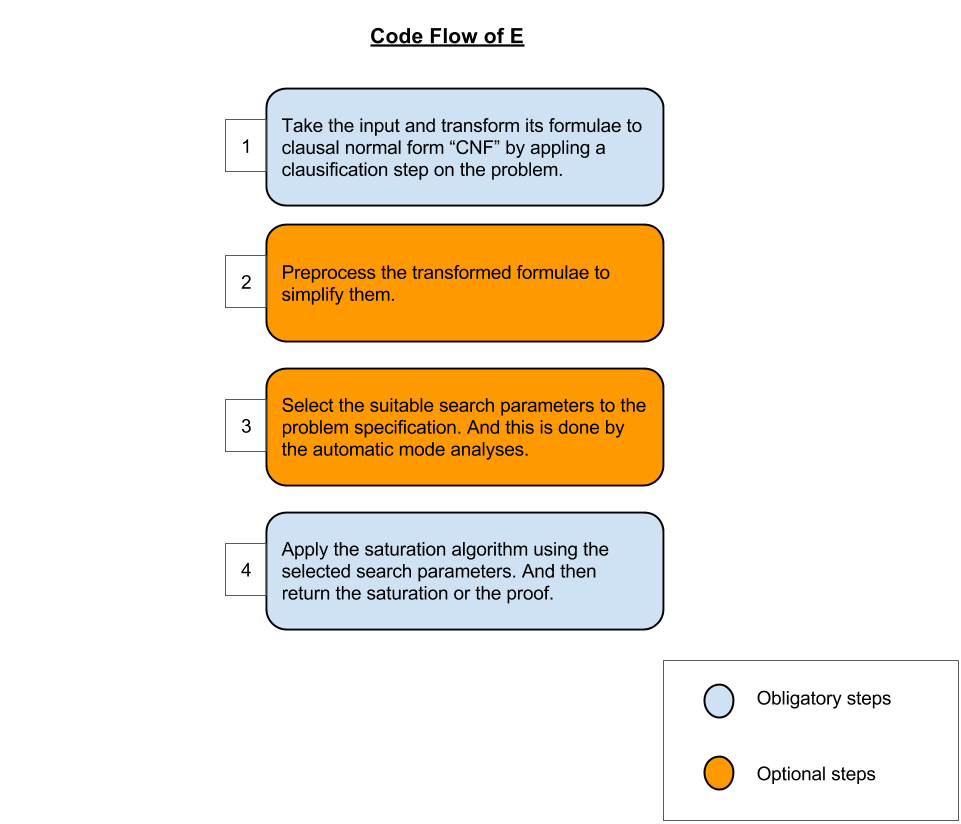
\includegraphics[scale=0.45]{pictures/e_code_flow.png}
		\caption{E Simplified code flow}\label{fig:e_code_flow}
	\end{figure}



\subsection{Latest results}
The latest results showed performance approaching 70\% over all the CNF and FOF problems of the TPTP problem set and this is according to \cite{E13}.



\section{Problem Set}
TPTP problems are first order problems, that are considered benchmarks to measure the performance of the different automated theorem provers. A description for TPTP could be found in \cite{TPTP09}, and the problem set could be downloaded from \url{http://www.cs.miami.edu/~tptp/}. TPTP problem set consists of different categories of problems, or divisions in other words, such as : PUZ, NLP, GRP. Those categories depends on the problems scientific meaning, e.g., NLP represents Natural language processing problems.


TPTP has its own language; TPTP for problems and TSTP for solutions. TPTP language could be written in two formats. The first of them is FOF, which is first order form. While the second form is CNF, which is clause normal form. Having a unified language for problems and solutions had a great impact on the field of \ac{atp}. And this allows the integration of different \ac{atp} systems ,i.e., Automated theorem provers, since they have a specific language that could communicate in.  


An example for a problem, i.e., GRP004-1 problem, from the TPTP problem set is given below in CNF format:

	\begin{lstlisting}[caption=GRP004-1.p problem,basicstyle=\footnotesize,breaklines=true,frame=single]
%--------------------------------------------------------------------------
% File     : GRP004-1 : TPTP v6.1.0. Released v1.0.0.
% Domain   : Group Theory
% Problem  : Left inverse and identity => Right inverse exists
% Version  : [Cha70] axioms : Incomplete.
% English  : In a group with left inverses and left identity every element
%            has a right inverse.

% Refs     : [Luc68] Luckham (1968), Some Tree-paring Strategies for Theore
%          : [Cha70] Chang (1970), The Unit Proof and the Input Proof in Th
%          : [CL73]  Chang & Lee (1973), Symbolic Logic and Mechanical Theo
% Source   : [Cha70]
% Names    : Example 3 [Luc68]
%          : Example 4 [Cha70]
%          : Example 4 [CL73]
%          : EX4 [SPRFN]

% Status   : Unsatisfiable
% Rating   : 0.00 v5.4.0, 0.11 v5.3.0, 0.10 v5.2.0, 0.00 v2.1.0, 0.00 v2.0.0
% Syntax   : Number of clauses     :    5 (   0 non-Horn;   3 unit;   3 RR)
%            Number of atoms       :   11 (   0 equality)
%            Maximal clause size   :    4 (   2 average)
%            Number of predicates  :    1 (   0 propositional; 3-3 arity)
%            Number of functors    :    3 (   2 constant; 0-1 arity)
%            Number of variables   :   15 (   1 singleton)
%            Maximal term depth    :    2 (   1 average)
% SPC      : CNF_UNS_RFO_NEQ_HRN

% Comments : [Luc68] is actually the right to left version.
%--------------------------------------------------------------------------
cnf(left_inverse,axiom,
    ( product(inverse(X),X,identity) )).
cnf(left_identity,axiom,
    ( product(identity,X,X) )).
cnf(associativity1,axiom,
    ( ~ product(X,Y,U)
    | ~ product(Y,Z,V)
    | ~ product(U,Z,W)
    | product(X,V,W) )).
cnf(associativity2,axiom,
    ( ~ product(X,Y,U)
    | ~ product(Y,Z,V)
    | ~ product(X,V,W)
    | product(U,Z,W) )).
cnf(prove_there_is_a_right_inverse,negated_conjecture,
    ( ~ product(a,X,identity) )).
%--------------------------------------------------------------------------
	\end{lstlisting}